\section{Theorie}
\label{sec:Theorie}
\subsection{Ziel des Versuches}
Es sollen die Eigenschaften und die Funktionsweisen eines Silizium-Halbleiterdetektors
mit diversen Aufgabenteilen genauer untersucht werden.

\subsection{Halbleiter}

Zuerst wird kurz auf die wichtigen Eigenschaften des Halbleiters eingegangen, da dieser
der wichtigste Bestandteil des Detektors ist. \\
Halbleiter sind Festkörper deren elektrische Leiteigenschaften zwischen elektrischen
Leitern und Nichtleitern liegen. Die Leiteigenschaften eines Materials wird mit
Hilfe des Bändermodells erklärt.

\begin{figure}[H]
  \centering
  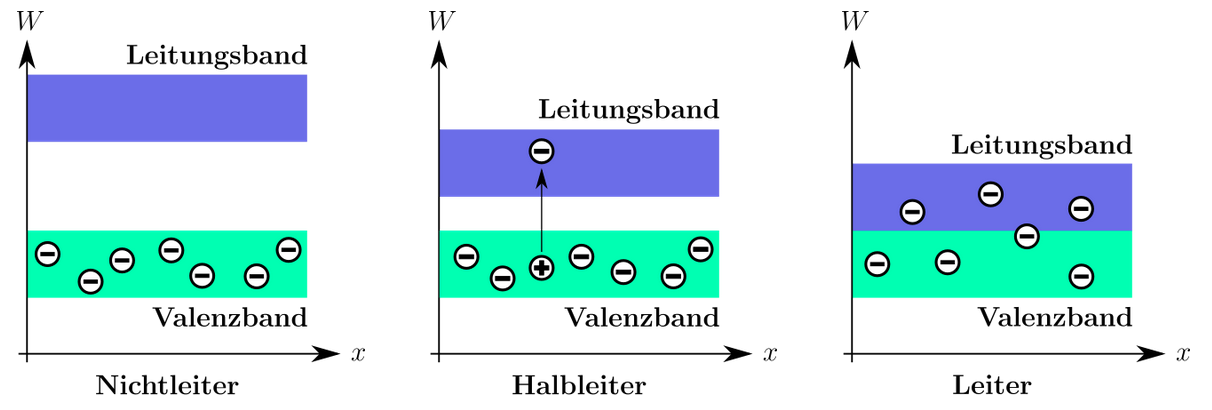
\includegraphics[width=1\textwidth]{ressources/halbleiter.png}
  \caption{Schematische Darstellung des Bändermodells}
  \label{bänder }
\end{figure}
Das Bändermodell unterteilt die Leitfähigkeit eines Materials in 3 Gruppen:
Leiter, Halbleiter und Isolatoren. Der Unterschied besteht in der Größe
der Bandlücke zwischen Leitungsband und Valenzband. Ist die Bandlücke groß,
so befinden sich keine Elektronen im Leitungsband und das Material ist ein Isolator. Überlappen
die Bänder, so spricht man von einem Leiter.
 Bei Halbleitern liegt die Bandlücke im Bereich $0,1$eV$<E<3$eV. Bei Temperaturen von über $0\,$K kommt es zu
Anregung von Elektronen und der Halbleiter besitzt leitende Eigenschaften.
 Des Weiteren werden Halbleiter in Element,-
Verbindungs,- und organische Halbleiter unterteilt. Innerhalb des Versuches wird
jedoch nur Silizium, also ein Elementhalbleiter, verwendet. Um die Leitfähigkeit
eines Halbleiters zu erhöhen können Fremdatome eingebracht werden, diesen Vorgang nennt man
Dotierung.
\subsection{p- und n- Halbleiter}
Der Elementhalbleiter Silizium gehört der vierten Hauptgruppe an und besitzt somit
vier Valenzelektronen. Zur Dotierung von Silizium eignen sich Atome mit drei oder
fünf Valenzelektronen. Dabei wird je nach Art der Dotierung zwischen
p-Typ (Dotierung mit Fremdatomen der dritten Hauptgruppe) und n-Typ (fünfte Hauptgruppe)
unterschieden.

Bei p-Typ Halbleitern wird ein Fremdatom der dritten Hauptgruppe eingefügt,
typische Dotierungsverhältnisse sind $10^{4-7}$ Si-Atome zu einem Fremdatom.
Durch die Dotierung fehlt ein Elektron in den kovalenten Bindungen, es entsteht ein
bewegliches Loch. Das Loch kann durch Elektroneneinfang wieder gefüllt werden,
deswegen werden solche Fremdatome auch als Akzeptoren bezeichnet.

Die n-Typ Halbleiter zeichnen sich durch eine Dotierung mit Elementen der
fünften Hauptgruppe aus. Bei einer solchen Dotierung entsteht ein Elektronenüberschuss
und pro dotiertes Fremdatom kommt es zu einem zusätzlichen Leitungselektron. Aufgrund
der Abgabe des Leitungselektron an das Gitter spricht man hier von einem Donator.

\subsection{Der pn- Übergang}
Bei einem pn-Übergang werden ein n- und ein p- dotierter Halbleiter verbunden.
Da die p-Seite einen Überschuss an Löchern und die n-dotierte Seite einen Überschuss an
Leitungselektronen hat kommt es in der Mitte zur Rekombination. Es bildet sich
eine Bereich in dem wenig Ladungsträger vorhanden sind. Dieser Bereich
wird Sperrschicht oder Depletionszone genannt. Ihre Dicke $d(U)$ hängt von der
dielektrischen Konstante des Halbleiters ab und kann mit
Hilfe der vorangelegten Spannung $U$ reguliert werden,
\begin{equation}
    \label{depl}
    d(U)=\sqrt{ \frac{ 2 \epsilon (U_D +U ) }{e N_\text{eff}}}.
\end{equation}
Des Weiteren hängt die Dicke von der Diffusionsspannung $U_D$ im dynamischen Gleichgewicht,
der Elementarladung e und von der Anzahl der effektiven Ladungsträgerdichte ab. Die
effektive Ladungsträgerdichte ist ein Verhältnis der Dotierungskonzentrationen von
Donatoren und Akzeptoren:
$$N_\text{eff}=\frac{N_D N_A}{N_D +N_A}$$


Um die später mit der Diode, welche aus einem pn-Übergang besteht, möglichst
gute Messungen zu erzielen ist es notwendig die Depletionszone über den gesamten
Kristall auszubreiten.  Dazu wird eine zusätzliche Spannung $U_\text{dep}$ angelegt.
Diese ist im Allgemeinen jedoch so klein $(U\ll U_\text{D})$, dass der Ausdruck \eqref{depl}
sich vereinfachen lässt zu:
\begin{equation}
    \label{dicke}
    d(U)=\sqrt{ \frac{ 2 \epsilon U }{e N_\text{eff}}}.
\end{equation}
Setzt man in diese Gleichung die Spannung $U_\text{dep}$ ein, so lässt sie sich umformen zu
\begin{equation}
    U_\text{dep}=\frac{q}{2 \epsilon} N_\text{eff}D^2,
\end{equation}
da bei Spannungen die $ U>U_\text{dep}$ die Dicke der Depletionszone der Sensordicke entspricht.
Für Spannungen von $U<U_\text{dep}$ gilt die Näherung:

\begin{equation}
    \label{depsu}
d(U)=D\sqrt{\frac{U}{U_\text{dep}}}
\end{equation}

\subsection{Pedestals und Noise}
Wie bei jeder elektronischen Messung haben wir Störsignale, die die Messung
verschlechtern. Diese Störsignale lassen sich nicht verhindern und werden $Noise$
genannt. In diesem Unterkapitel wird darauf eingegangen wie man das Rauschen
minimieren kann. Dazu betrachten wir zuerst das Signal, welches
zum Beispiel auf einem Streifen ($i$) eines Silizium-Detektors gemessen wird.
Die gemessenen Counts für ein Signal $k$ werden ADC($i,k$) Counts bezeichnet.
\begin{equation}
\label{ADC}
\text{ADC}(i,k)=P(i,k)+D(k)+\text{Signal}(i,k)
\end{equation}
Betrachtet man nun den Mittelwert der ADC Counts eines Streifen ohne externes Signal$(i,k)$,
so wird dieses als Pedestal bezeichnet. Es beschreibt also das Grundrauschen eines Streifen ohne
Messungen von externen Signalen. Er ergibt sich als:
\begin{equation}
    \label{peds}
    \text{P}(i)=\frac{1}{N}\sum_i^{N} \text{ADC}(i,k).
\end{equation}
Wobei $N$ die Anzahl der durchgeführten Messungen ist.
Bei einer Messung eines Signals kommt es neben dem schon oben diskutierten $Noise$
noch zu einer Weiteren Störquelle, dem $Common \,\,Mode \,\,Shift$. Bei einem Detektor mit
128 Streifen lässt sich der $Common \,\,Mode \,\,Shift\,\, \text{D}(k)$ wie folgt ermitteln:
\begin{equation}
    \label{common}
    D(k)=\frac{1}{128}\sum_{i=1}^{128}(ADC(i,k)-P(i)).
\end{equation}
Das $Noise$ der einzelnen Streifen kann über den $RMS\,$(root mean square)
der ADC Counts nach Abzug der Pedestals und des Common Mode Shifts bestimmt werden.
\begin{equation}
    \label{noise}
    \text{Noise}=\sqrt{\frac{1}{N-1}\sum_{k=1}^{N}( \text{ADC}(i,k)-\text{P}(i)-\text{D}(k))^2. }
\end{equation}
% 2x2 Plot
% \begin{figure*}
%     \centering
%     \begin{subfigure}[b]{0.475\textwidth}
%         \centering
%         \includegraphics[width=\textwidth]{Abbildungen/Schaltung1.pdf}
%         \caption[]%
%         {{\small Schaltung 1.}}
%         \label{fig:Schaltung1}
%     \end{subfigure}
%     \hfill
%     \begin{subfigure}[b]{0.475\textwidth}
%         \centering
%         \includegraphics[width=\textwidth]{Abbildungen/Schaltung2.pdf}
%         \caption[]%
%         {{\small Schaltung 2.}}
%         \label{fig:Schaltung2}
%     \end{subfigure}
%     \vskip\baselineskip
%     \begin{subfigure}[b]{0.475\textwidth}
%         \centering
%         \includegraphics[width=\textwidth]{Abbildungen/Schaltung4.pdf}    % Zahlen vertauscht ... -.-
%         \caption[]%
%         {{\small Schaltung 3.}}
%         \label{fig:Schaltung3}
%     \end{subfigure}
%     \quad
%     \begin{subfigure}[b]{0.475\textwidth}
%         \centering
%         \includegraphics[width=\textwidth]{Abbildungen/Schaltung3.pdf}
%         \caption[]%
%         {{\small Schaltung 4.}}
%         \label{fig:Schaltung4}
%     \end{subfigure}
%     \caption[]
%     {Ersatzschaltbilder der verschiedenen Teilaufgaben.}
%     \label{fig:Schaltungen}
% \end{figure*}
